\documentclass[10pt,a4paper]{report}
\usepackage[utf8]{inputenc}
\usepackage{graphicx}
\usepackage{color}
\usepackage{subcaption}
\usepackage{mathtools}
\usepackage{cite}
\usepackage[export]{adjustbox}
\usepackage[table]{xcolor}
\usepackage{amsmath}


\title{LaTex project}
\author{Almasyan Sanasar}
\date{July 2022}

\begin{document}
\maketitle

\begin{abstract}
\textsf{friends! Further development of different types of activity makes it possible to assess the importance of the development model. A rich variety of experience with the implementation of planned goals provides a wide range of (expert) participation in the development model. However, we must not forget that the current structure of the organization requires us to analyze the methods of mass participation.
\\\texttt{,,3th of August, 19:00, club RNDM`} }
\end{abstract}

\tableofcontents
\chapter{Random text and images}
\section{Text}
Lorem ipsum dolor sit amet. Sit voluptatum cupiditate et neque modi et totam nihil vel voluptas nihil ut consequatur exercitationem et\footnote{idk just a footenote} assumenda autem ut perspiciatis quas. Est nisi amet aut facere unde voluptates commodi ab Quis dolor aut dicta minus aut deserunt unde ut facere tenetur.\cite{chen2001one}

Sit alias dolorum non alias nobis est quasi quidem ea voluptas Quis et repellendus sint. Ea veniam fuga id ipsa quod in laborum incidunt sit magni enim!

Est fuga quae et ullam quam et pariatur nihil rem enim soluta aut voluptatem laudantium. Qui officiis exercitationem est numquam labore eum consectetur excepturi. Ab cumque tempore quo eveniet rerum nam enim praesentium et voluptas natus id perspiciatis dolor et voluptas temporibus et quam maiores.\cite{cherkassky2004practical}
\begin{figure}
    \centering
    \begin{subfigure}{0.3\textwidth}
    \label{fig:sub1}
    \end{subfigure}
    \begin{subfigure}{0.3\textwidth}
    \label{fig:sub2}
    \end{subfigure}
    \begin{subfigure}{0.3\textwidth}
    \label{fig:sub3}
    \end{subfigure}
\end{figure}
\clearpage

\section{Images}
\begin{center}
\end{center}
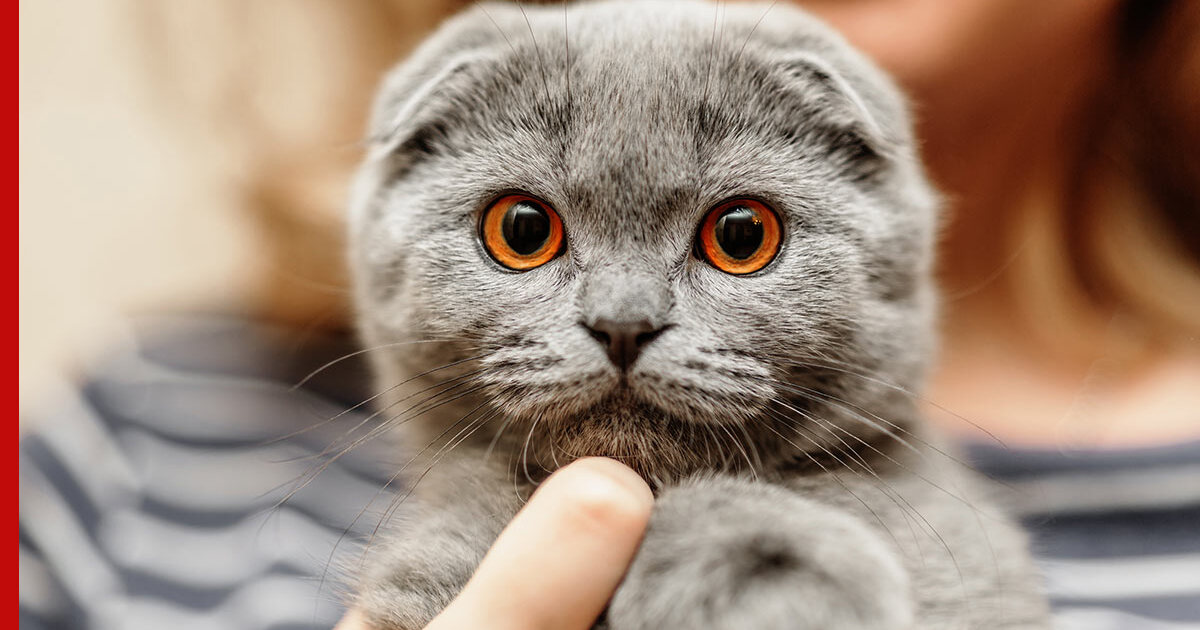
\includegraphics[width=0.7\linewidth, right]{photos/906045-fb.jpeg}
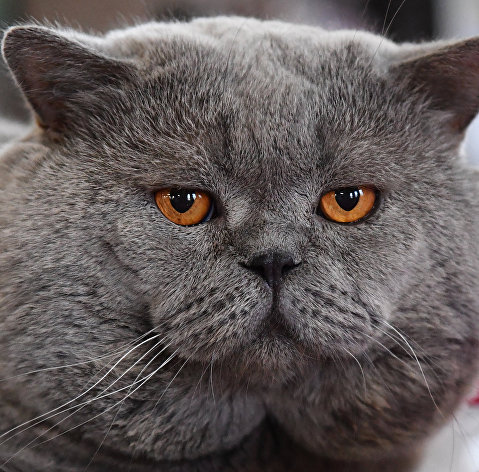
\includegraphics[width=0.7\linewidth, right]{photos/834107650.jpg}

\begin{figure}[h]
    \centering
    \begin{subfigure}{0.3\textwidth}
    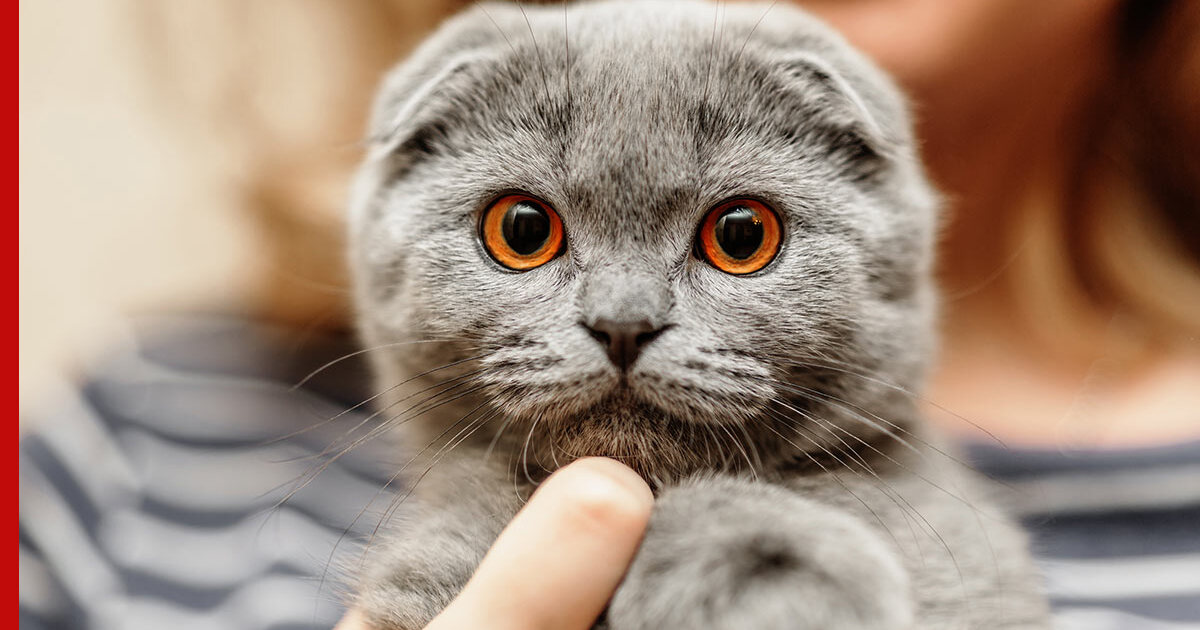
\includegraphics[width=1\linewidth, height=4cm]{photos/906045-fb.jpeg}
    \caption{example 1}
    \label{fig:sub1}
    \end{subfigure}
    \begin{subfigure}{0.3\textwidth}
    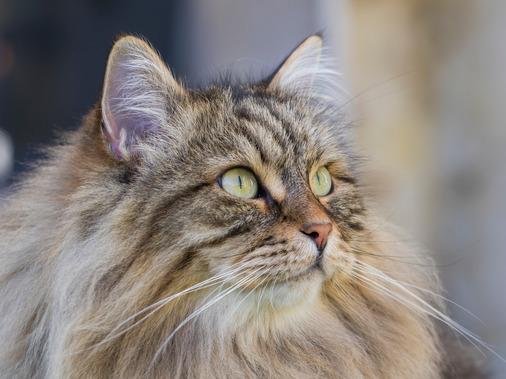
\includegraphics[width=1\linewidth, height=4cm]{photos/MicrosoftTeams-image (6) (1)_1.jpg}
    \caption{example 2}
    \label{fig:sub2}
    \end{subfigure}
    \begin{subfigure}{0.3\textwidth}
    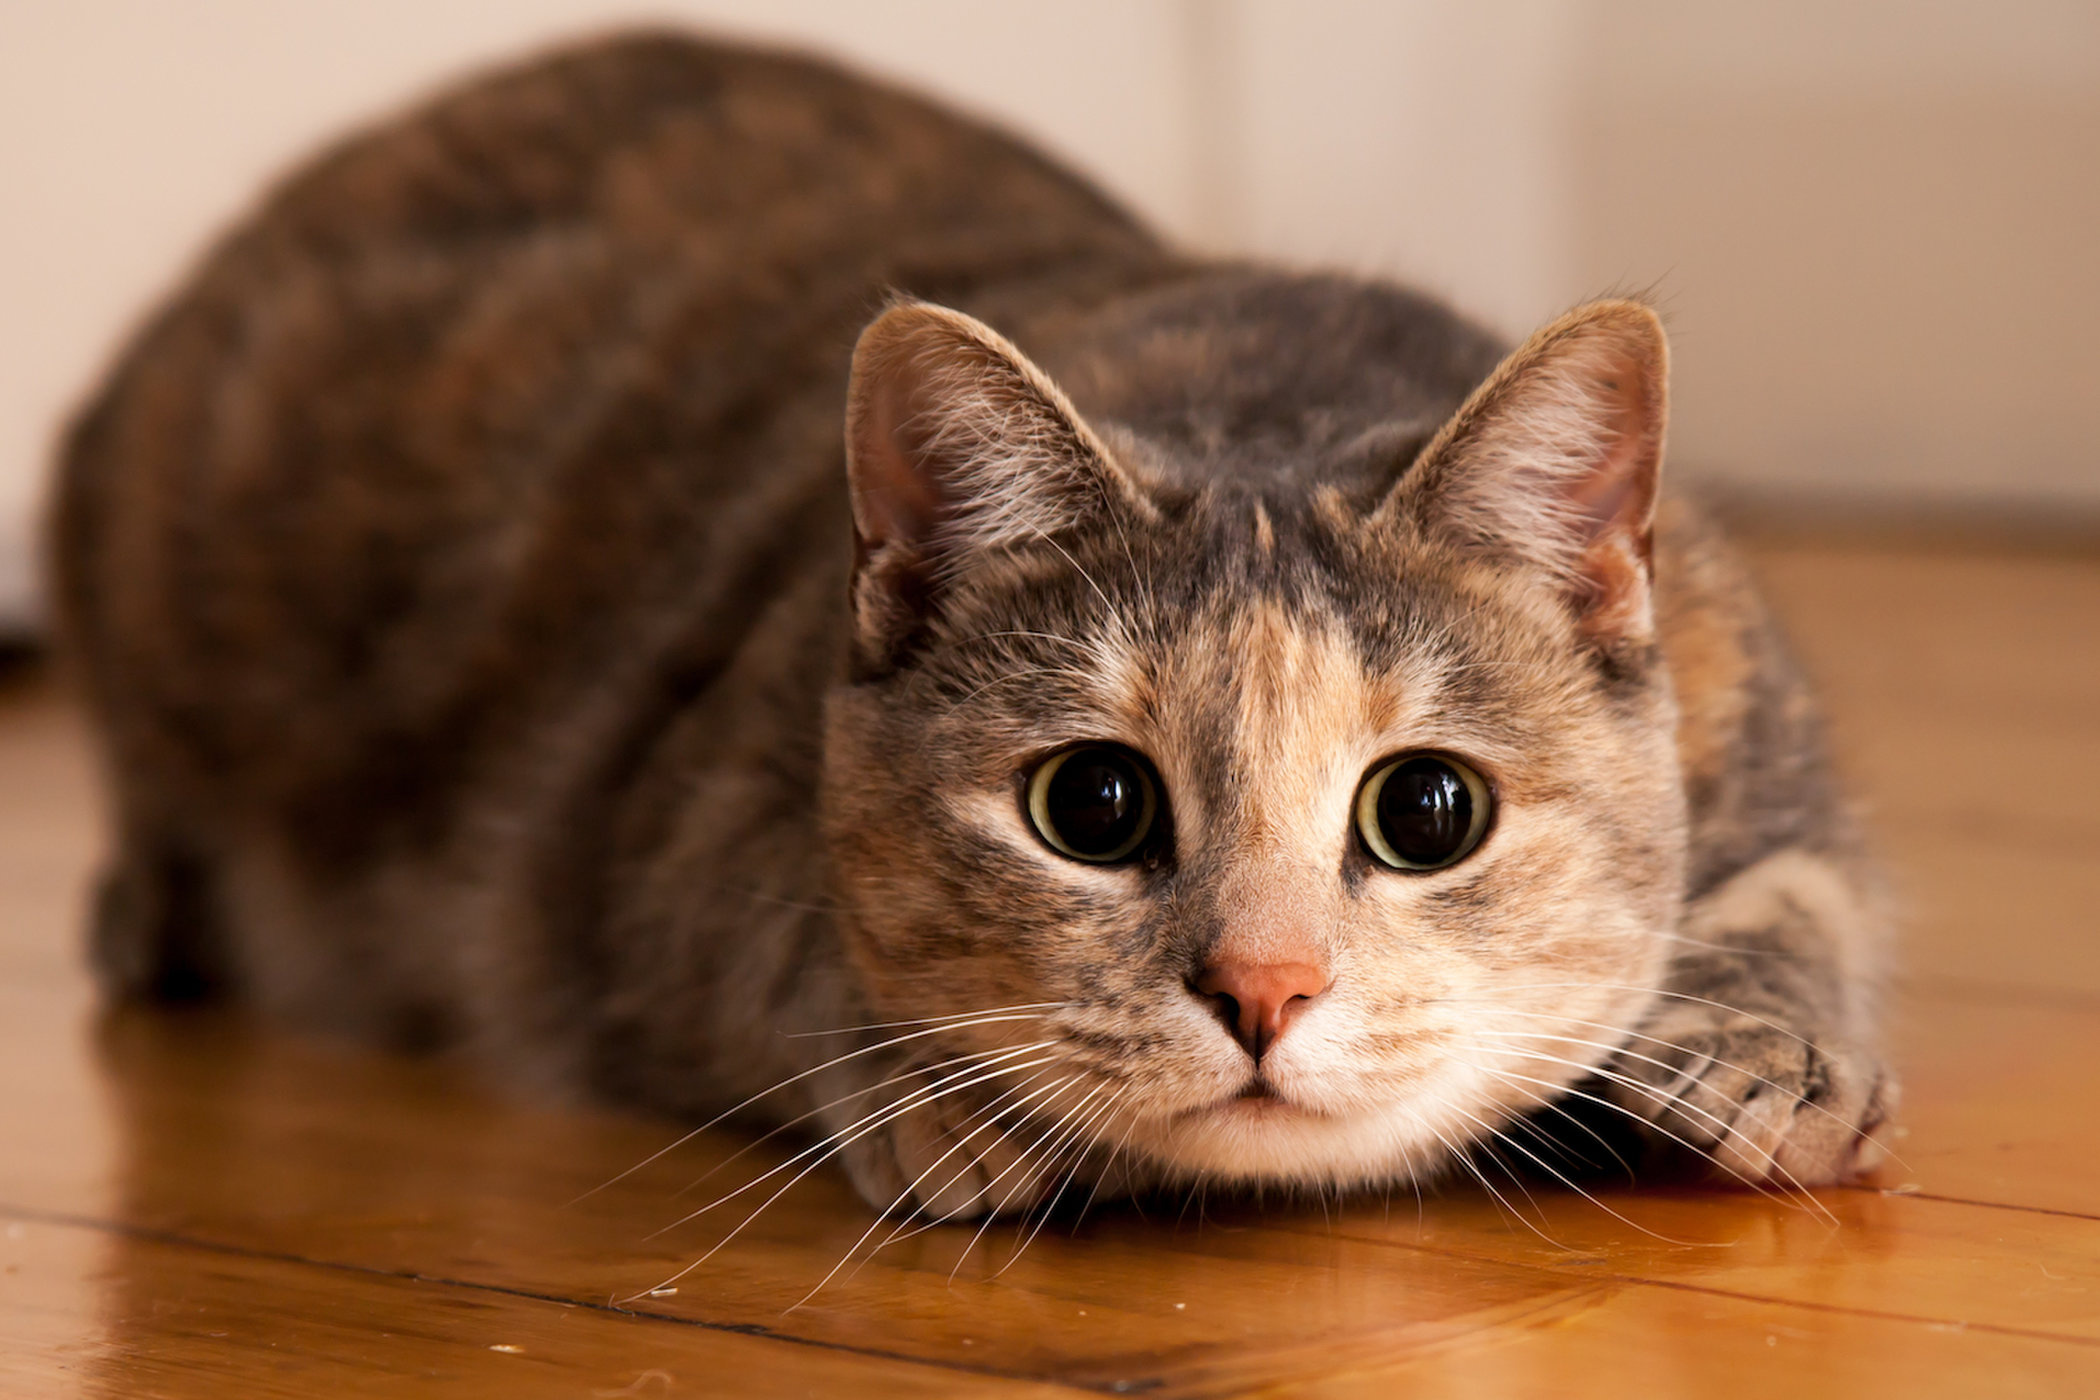
\includegraphics[width=1\linewidth, height=4cm]{photos/aHR0cDovL3d3dy5saXZlc2N.jpg}
    \caption{example 3}
    \label{fig:sub3}
    \end{subfigure}
    \caption{This is a caption}
\caption{}
\label{fig:figure1}
\end{figure} 

\chapter{Maths}
\section{Formulas}
\begin{align}
    Y_{ij} = \begin{dcases*}
        \sum_{k \sim i}y_{ij}, & if $ i = j $,\\
        {-y_{ij}}, & if $ i \ne j $ and $ i \sim j $,\\
        0, & otherwise. 
        \end{dcases*}
\end{align}
\\
\\
\\
\begin{align}
    \begin{split}
      V &= \iiint \rho^{2} sin{\theta} d\rho d\theta d\varphi \\
      &= \int_{0}^{2\pi} \int_{0}^{\pi} \int_{0}^{r} \rho^{2} \sin{\theta} d\rho d\theta d\varphi \\
      &= 2\pi \int_{0}^{\pi} \int_{0}^{r} \rho^{2} \sin{\theta} d\rho d\theta \\
      &= 4\pi \int_{0}^{r} \rho^{2} d\rho \\
      &= \frac{4\pi}{3}\rho^{3}
    \end{split}
\end{align}
\begin{math}
\int{\frac{\sec{x}^4}{8 \cdot \sqrt{7 - 6 \cdot \tan{x} - \tan{x}^2}}\,dx}
\end{math}
\\
\\
\\


\[ x^n + y^n = z^n \]


$ \forall x \in X, \quad \exists y \leq \epsilon $

$ \frac{n!}{k!(n-k)!} = \binom{n}{k} $

$$ \forall x \in X, \quad \exists y \leq \epsilon $$


\begin{math}
x^n + y^n = z^n 
\end{math}

\begin{center}

$ \forall x \in X, \quad \exists y \leq \epsilon $

$$ \cos(2\theta) = \cos^2 \theta - \sin^2 \theta $$

$ \lim\limits_{x \to \infty} \exp(-x) = 0 $

$ \frac{n!}{k!(n-k)!} = \binom{n}{k} $

$ \frac{\frac{1}{x}+\frac{1}{y}}{y-z} $

$$ ^3/_7 $$
$$ 78 \cdot 89 $$
\end{center}

\begin{equation}\label{eq:x}
  x = a_0 + \cfrac{1}{a_1 
          + \cfrac{1}{a_2 
          + \cfrac{1}{a_3 + \cfrac{1}{a_4} } } }
\end{equation}


Text and \ref{eq:x}
\\

$ 6 \cdot 6$

% https://ru.overleaf.com/learn/latex/Matrices#amsmath_matrix_environments
$$\begin{matrix}
1 & 2 & 3\\
a & b & c
\end{matrix}$$

$$\begin{pmatrix}
1 & 2 & 3\\
a & b & c
\end{pmatrix}$$

$ A_{m,n} = 
 \begin{pmatrix}
  a_{1,1} & a_{1,2} & \cdots & a_{1,n} \\
  a_{2,1} & a_{2,2} & \cdots & a_{2,n} \\
  \vdots  & \vdots  & \ddots & \vdots  \\
  a_{m,1} & a_{m,2} & \cdots & a_{m,n} 
 \end{pmatrix} $ \\
 \\
 \\
 \\
 \begin{equation}
  L' = {L}{\sqrt{1-\frac{v^2}{c^2}}}
 \end{equation}
\clearpage
\section{Lists}
Unordered list
\begin{itemize}
    \item 1 cow
    \item 2 cows
    \item 3 cows
\end{itemize} 
Ordered list
\begin{enumerate}
    \item 1 ape
    \item 2 apes
    \item 3 apes
\end{enumerate}
Nested list
\begin{enumerate}
    \item Family 1
    \begin{enumerate}
        \item Papa
        \item Mama
        \item Sobaka
    \end{enumerate}
    \item Single 1
    \item Single 2
    \end{enumerate}

\clearpage
\chapter{The rest}
\section{Tables}
\begin{center}
\rowcolors{1}{yellow}{pink}
\begin{tabular}{||c c c c||} 
 \hline
 Col1 & Col2 & Col2 & Col3 \\ [1ex] 
 \hline\hline
 322 & 228 & 1337 & 1769 \\ 
 \hline
 1234 & 2 & 3 & 4 \\
 \hline
 6 & 7 & 88 & 99 \\
 \hline
 213 & 231 & 321 & 123 \\
 \hline
 123 & 423 & 5428 & 2123 \\ [1ex] 
 \hline
\end{tabular}
\end{center}
\begin{tabular}{ |p{2cm}||p{2cm}|p{2cm}|p{2cm}|  }
 \hline
 \multicolumn{4}{|c|}{Names} \\
 \hline
 Russia& USA&Armenia&Kazakhstan\\
 \hline
 Pasha  & John    &Sanasar&   Adil\\
 Sashas&   Josh  & Bagdasar & Kadir\\
 Dasha &Joe & Ruslan&  Davlet\\
 \hline
\end{tabular}

\bibliographystyle{plain}
\bibliography{bib.bib}
  
\end{document} 



